% Fig. 1 of tit-stationary.tex: the three parties.  Build: pdflatex fig_model.tex
\documentclass[border=3pt]{standalone}
\usepackage{amsmath,amssymb}
\renewcommand{\rmdefault}{ptm}% Times text, as in IEEEtran
\usepackage{tikz}
\usetikzlibrary{positioning,arrows.meta,calc}
\begin{document}
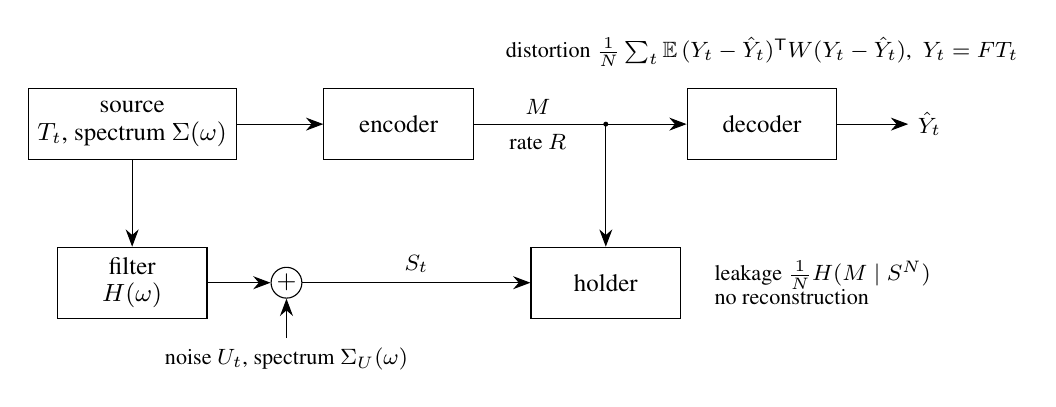
\begin{tikzpicture}[
  >={Stealth[length=2.2mm]},
  box/.style={draw, minimum height=9mm, minimum width=19mm, align=center, font=\small},
  lab/.style={font=\footnotesize, align=center},
]
% the description
\node[box] (src) {source\\[-1pt]$T_t$, spectrum $\Sigma(\omega)$};
\node[box, right=11mm of src] (enc) {encoder};
\node[box, right=27mm of enc] (dec) {decoder};
\node[right=9mm of dec, lab] (yh) {$\hat Y_t$};
\draw[->] (src) -- (enc);
\draw[->] (enc) -- node[pos=0.3, above, lab] {$M$} node[pos=0.3, below, lab] {rate $R$} (dec);
\draw[->] (dec) -- (yh);
\node[lab, above=1.5mm of dec] {distortion $\tfrac1N\sum_t\mathbb E\,(Y_t-\hat Y_t)^{\mathsf T}W(Y_t-\hat Y_t)$,\ \ $Y_t=FT_t$};
% the holder's observation
\node[box, below=11mm of src] (filt) {filter\\[-1pt]$H(\omega)$};
\node[draw, circle, inner sep=0.6pt, right=8mm of filt, font=\small] (plus) {$+$};
\node[lab, below=5mm of plus] (noise) {noise $U_t$, spectrum $\Sigma_U(\omega)$};
\coordinate (tap) at ($(enc.east)!0.62!(dec.west)$);
\node[box] (hold) at (tap |- filt) {holder};
\draw[->] (src) -- (filt);
\draw[->] (filt) -- (plus);
\draw[->] (noise) -- (plus);
\draw[->] (plus) -- node[above, lab] {$S_t$} (hold);
\fill (tap) circle (0.9pt);
\draw[->] (tap) -- (hold.north);
\node[lab, right=3mm of hold, align=left] {leakage $\tfrac1N H(M\mid S^N)$\\[-1pt]no reconstruction};
\end{tikzpicture}
\end{document}
